\documentclass{beamer}
\usepackage{geometry}
\usepackage[english]{babel}
\usepackage[utf8]{inputenc}
\usepackage{amsmath}
\usepackage{amsfonts}
\usepackage{amssymb}
\usepackage{tikz}
\usetikzlibrary{quotes, angles}
\usepackage{graphicx}

%\usepackage{pgfplots}
%\pgfplotsset{width=10cm,compat=1.9}
%\usepackage{pgfplotstable}

\setlength{\headheight}{26pt}%doesn't seem to fix warning

\usepackage{fancyhdr}
\pagestyle{fancy}
\fancyhf{}

%\rhead{\small{2 January 2019}}
\lhead{\small{BECA / Dr. Huson / Geometry - Unit 7 Analytic Geometry}}

\renewcommand{\headrulewidth}{0pt}

\title{10th Grade Geometry - Unit 7: Analytic Geometry}
\subtitle{Bronx Early College Academy}
\author{Christopher J. Huson PhD}
\date{29 January - 1 March 2019}

\begin{document}
\frame{\titlepage}
\section[Outline]{}
\frame{\tableofcontents}


\section{Seating Chart 10.1}
  \frame
  {
    \frametitle{Seating Chart 10.1}
    \framesubtitle{How do we work as a team?}

    %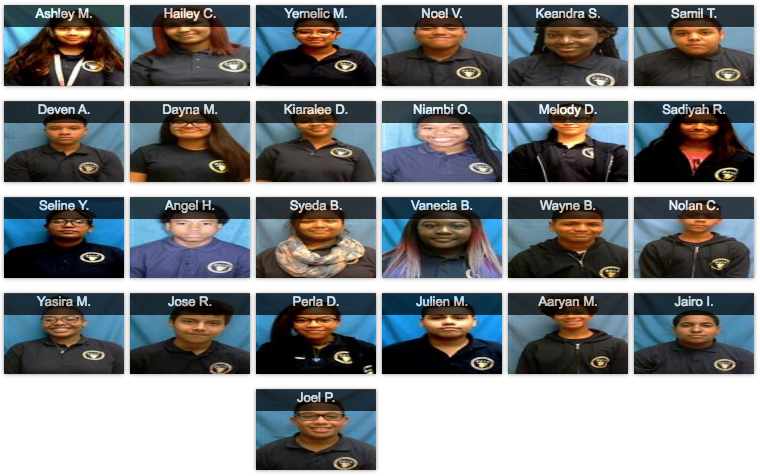
\includegraphics[width=1.0\textwidth]{seating-10A.png}
  }

\section{Seating Chart 10.2}
  \frame
  {
    \frametitle{Seating Chart 10.2}
    \framesubtitle{How do we work as a team?}

    %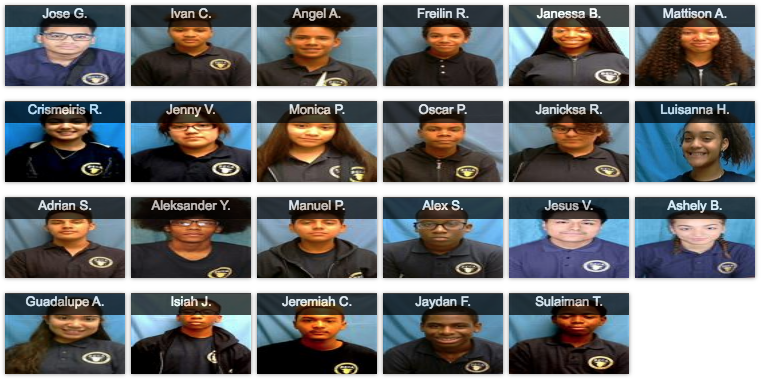
\includegraphics[width=1.0\textwidth]{seating-10B.png}
  }

\section{7.1 Laptops - Geogebra. Tuesday 28 January}
  \frame
  {
    \frametitle{GQ: How do we model with digital tools?}
    \framesubtitle{CCSS: HSG.CO.D.12 Congruence, geometric constructions \hspace{\stretch{1}} \alert{7.1 Tuesday 18 January}}

    \begin{block}{Do Now: Regents review and reflection}
      \begin{itemize}
        \item Results: 10 passing scores, 4 college ready
        \item Top score 75; average 53
        \item 70\% earned free response points
      \end{itemize}
    \end{block}
    GeoGebra Geometry App\\
    Enter \alert{N7BHK} for 10.1 or \alert{P9PNZ} for 10.2\\
    Set up account using your real name.\\
    Beginner Tutorials with Lesson Ideas\\
    Author: Tim Brzezinski\\[0.5cm]
    Homework: Complete Geogebra
  }

\section{7.2 Linear equations. Wednesday 30 January}
  \frame
  {
    \frametitle{GQ: How do we use functions and equations to represent objects on the coordinate plane?}
    \framesubtitle{CCSS: HSG.CO.D.12 Congruence, geometric constructions \hspace{\stretch{1}} \alert{7.2 Wednesday 30 January}}

    \begin{block}{Do Now: Handout}
      \begin{enumerate}
        \item Dilation, plotting equations
      \end{enumerate}
    \end{block}
    Function notation, slope-intercept, standard, \& point slope forms of linear equations\\[0.5cm]
    Homework: Handout review of linear equations and functions
  }

\section{7.3 Linear equations. Thursday 31 January (cold day)}
  \frame
  {
    \frametitle{GQ: How do we use functions and equations to represent objects on the coordinate plane?}
    \framesubtitle{CCSS: HSG.CO.D.12 Congruence, geometric constructions \hspace{\stretch{1}} \alert{7.3 Thursday 31 January}}

    \begin{block}{Do Now: Handout}
      \begin{enumerate}
        \item Translation, plotting equations
      \end{enumerate}
    \end{block}
    Function notation, slope-intercept, standard, \& point slope forms of linear equations\\[0.5cm]
    Homework: Handout review of linear equations and functions
  }

\section{7.4 Slope applications in proof. Friday 1 February}
\frame
{
\frametitle{GQ: How do we use slope in geometric proof?}
\framesubtitle{CCSS: HSG.CO.D.12 Congruence, geometric constructions \hspace{\stretch{1}} \alert{7.4 Friday 1 February}}

\begin{block}{Do Now: Handout}
  \begin{enumerate}
    \item Translating segments, plotting equations, perpendicular proof
  \end{enumerate}
\end{block}
Applying slope to prove parallel or perpendicular relationships\\[0.5cm]
Homework: Handout review of linear \& quadratic equations and functions
}

\section{7.5 Function translation. Monday 4 February}
\frame
{
  \frametitle{GQ: How do we apply translations to functions?}
  \framesubtitle{CCSS: HSG.CO.D.12 Congruence, geometric constructions \hfill \alert{7.5 Monday 4 February}}

  \begin{block}{Do Now: Handout}
    \begin{enumerate}
      \item Translating segments, plotting equations, perpendicular proof
    \end{enumerate}
  \end{block}
  Translating parabolas, vertex form\\[0.5cm]
  Homework: Pretest for review Wednesday. \alert{Test Thursday}
}

\section{7.6 Function translation. Wednesday 6 February}
  \frame
  {
    \frametitle{GQ: How do we apply translations to functions?}
    \framesubtitle{CCSS: HSG.CO.D.12 Congruence, geometric constructions \hfill \alert{7.6 Wednesday 6 February}}

    \begin{block}{Do Now: Handout}
      \begin{enumerate}
        \item Translating segments, plotting quadratics
      \end{enumerate}
    \end{block}
    Translating parabolas, vertex form\\[0.5cm]
    Homework: Study for \alert{test tomorrow}
  }

\section{7.7 Test. Thursday 7 February}
  \frame
  {
    \frametitle{GQ: How do we apply translations to functions?}
    \framesubtitle{CCSS: HSG.CO.D.12 Congruence, geometric constructions \hfill \alert{7.7 Thursday 7 6 February}}


    Assessment: Unit Test\\[0.5cm]
    Homework: Financial Mathematics handout
  }

\section{7.8 Financial math, Benjamin Segal. Friday 8 February}
  \frame
  {
    \frametitle{GQ: How do we use mathematics in business?}
    \framesubtitle{CCSS: MP. 4 Modeling with mathematics \hfill \alert{7.8 Friday 8 February}}
    Welcome guest instructor Mr. Segal, Neuberger Berman\\[0.5cm]
    \begin{block}{Do Now: Answer these questions in your notebook}
      \begin{enumerate}
        \item How much profit does Apple make on each i-phone it sells? (approximately)
        \item Do they make more on an i-phone, i-pad, or Mac computer?
        \item Is Apple stock a good investment? Justify your answer.
      \end{enumerate}
    \end{block}
    Lesson: Modeling the financial results of Apple Inc.\\[0.5cm]
    Homework: Practice problems
  }

\section{7.9 Completing the square. Monday 11 February}
  \frame
  {
    \frametitle{GQ: How do we apply translations to functions?}
    \framesubtitle{CCSS: HSG.CO.D.12 Congruence, geometric constructions \hfill \alert{7.9 Monday 11 February}}

    \begin{block}{Geogebra project: Handout}
      \begin{enumerate}
        \item Right triangles' side lengths satisfy $a^2+b^2=c^2$
        \item Pythagorean triples are integers that satisfy $a^2+b^2=c^2$\\
        \begin{tabular}{lll}
          & 3, 4, 5 &  5, 12, 13 \\
          6, 8, 10 & 8, 15, 17 & 7, 24, 25
        \end{tabular}
      \end{enumerate}
    \end{block}
    Homework review, the equation of a circle\\
    Lesson: Completing the square, efficient algebra techniques\\[0.5cm]
    Homework: Practice problems handout
  }

\section{7.10 Geogegra transformations intro. Tuesday 12 February}
  \frame
  {
    \frametitle{GQ: How do we apply translations to functions?}
    \framesubtitle{CCSS: HSG.CO.D.12 Congruence, geometric constructions \hfill \alert{7.10 Tuesday 12 February}}

    \begin{block}{Geogebra project: Create a transformations puzzle problem}
      \begin{enumerate}
        \item Start with a polygon
        \item Use Geogebra's tranformations tools
        \item List the transformation steps you used
        \item Rubric: correct, aesthetics, MLA
        \item Print out a color pdf to email me. (husonbeca@gmail.com)
      \end{enumerate}
    \end{block}
    Lesson: Geogebra tool pallette\\[0.5cm]
    Homework: Practice problems
  }

\section{7.11 Circle equations, simplifying radicals. Wednesday 13 February}
  \frame
  {
    \frametitle{GQ: How do we work with radicals?}
    \framesubtitle{CCSS: HSG.CO.D.12 Congruence, geometric constructions \hfill \alert{7.11 Wednesday 13 February}}

    \begin{block}{Do Now: Complete the square by adding a constant, then factor as a binomial squared}
      \begin{enumerate}
        \item Example: $x^2+6x \rightarrow$ \qquad $x^2+6x+9=(x+3)^2$
        \item $x^2+10x \rightarrow$
        \item $x^2+12x \rightarrow$
        \item $x^2-8x \rightarrow$
      \end{enumerate}
    \end{block}
    Simplify radicals: $\sqrt{12}$\\
    Lesson: Completing the square, circles p. 798, simplifying radicals\\
    Classwork: Textbook problems 9-35 odds p. 801\\[0.5cm]
    Homework: Practice problems handout
  }

\section{7.12 Distance proofs. Thursday 14 February}
  %duplicated class due to school event, Thursday-Friday
  \frame
  {
    \frametitle{GQ: How do we use distance in proofs?}
    \framesubtitle{CCSS: HSG.CO.D.12 Congruence, geometric constructions \hfill \alert{7.12 Thursday 14 February}}

    \begin{block}{Do Now Quiz}
      \begin{enumerate}
        \item Operations on the coordinate plane
        \item Applications of slope, graphing linear equations
        \item The equation of a circle, deriving center and radius
      \end{enumerate}
    \end{block}
    Lesson: Completing the square, efficient algebra techniques\\[0.5cm]
    Homework: Practice problems handout
  }

\section{7.13 Review. Friday 15 February}
  \frame
  {
    \frametitle{GQ: How do we use algebra in geometry problems?}
    \framesubtitle{CCSS: HSG.CO.D.12 Congruence, geometric constructions \hfill \alert{7.13 Friday 15 February}}

    \begin{block}{Do Now Quiz}
      \begin{enumerate}
        \item Operations on the coordinate plane
        \item Applications of slope, graphing linear equations
        \item The equation of a circle, deriving center and radius
      \end{enumerate}
    \end{block}
    Lesson: Completing the square, efficient algebra techniques\\[0.5cm]
    %Lesson: equations defining other conics\\[0.5cm]
    Homework: Practice problems handout
  }

\section{7.14 Triangle midlines, medians. Monday 25 February}
  \frame
  {
    \frametitle{GQ: How do we use triangle midlines?}
    \framesubtitle{CCSS: HSG.CO.D.12 Congruence, geometric constructions \hfill \alert{7.14 Monday 25 February}}

    \begin{block}{Do Now Analytic geometry review}
      \begin{enumerate}
        \item Point-slope form of linear equations
        \item Applications of slope, graphing linear equations
        \item The equation of a circle, deriving center and radius
      \end{enumerate}
    \end{block}
    Lesson: Midlines, medians, the centroid. Measuring with Geogebra, submissions standards\\[0.5cm]
    Homework: Practice problems handout
  }

\section{7.15 Geogegra median partition 2:1 ratio. Tuesday 26 February}
  \frame
  {
    \frametitle{GQ: How do we use technology to explore geometric relationships?}
    \framesubtitle{CCSS: MP5 Use appropriate tools strategically: dynamic geometry software \hfill \alert{7.15 Tuesday 26 February}}

    Do Now: Practice analytic geometry skills on handout
    \begin{block}{Lesson: Geogebra project to measure the division of a median of a triangle by the centroid}
      \begin{enumerate}
        \item Start with a triangle, connect two midpoints and medians, intersecting at the centroid
        \item Use Geogebra's measurement tools
        \item Explain the resulting 2:1 ratio using text and symbols
        \item Assessment rubric: correct, aesthetics, MLA
        \item Print out a color pdf to email me. (husonbeca@gmail.com)
      \end{enumerate}
    \end{block}
    Homework: Pretest packet due Thursday \alert{(test Friday)}
    %Multiple choice test? TestWizard
  }

\section{7.16 Analytics pretest review. Thursday 28 February}
  \frame
  {
    \frametitle{GQ: How do we apply algebra to geometric situations?}
    \framesubtitle{CCSS: HSG.CO.D.12 Congruence, geometric constructions \hfill \alert{7.16 Thursday 28 February}}

    \begin{block}{Do Now Analytic geometry review}
      \begin{enumerate}
        \item Point-slope form of linear equations
        \item Applications of slope, graphing linear equations
        \item The equation of a circle, deriving center and radius
      \end{enumerate}
    \end{block}
    Lesson: Pretest packet homework review\\[0.5cm]
    Homework: Study for \alert{test tomorrow}
  }

\section{7.17 Analytic geometry test. Friday 1 March}
  \frame
  {
    \frametitle{GQ: How do we apply translations to functions?}
    \framesubtitle{CCSS: HSG.CO.D.12 Congruence, geometric constructions \hfill \alert{7.17 Friday 1 March}}

    Assessment: Unit Test\\[0.5cm]
    Homework: Coordinate geometry handout
  }


\section{7.18 Geogegra - ?. Tuesday 5 March}
  \frame
  {
    \frametitle{GQ: How do we use technology to explore geometric relationships?}
    \framesubtitle{CCSS: MP5 Use appropriate tools strategically: dynamic geometry software \hfill \alert{7.19 Tuesday 6 March}}

    Do Now: Practice analytic geometry skills on handout
    \begin{block}{Lesson: Geogebra project to measure the division of a median of a triangle by the centroid}
      \begin{enumerate}
        \item Start with a triangle, connect two midpoints and medians, intersecting at the centroid
        \item Use Geogebra's measurement tools
        \item Explain the resulting 2:1 ratio using text and symbols
        \item Assessment rubric: correct, aesthetics, MLA
        \item Print out a color pdf to email me. (husonbeca@gmail.com)
        \item Filename: Last-First_Title.png, email subject line \& message
      \end{enumerate}
    \end{block}
    \alert{Parent conferences this Thursday evening, Friday afternoon}\\
    Homework:
  }



\end{document}
